\begin{frame}{もろもろ作成}
   \begin{columns}[t]
    \begin{column}{0.6\textwidth}
      <もろもろ作成の概要>
      \begin{itemize}
        \item[(1)]<1->  材質の作成 \\
		       「Material」を右クリックし「create」\\
		       「Elasticity」→「Elastic」を選択\\
		        ヤング率を206000[MPa]に \\
		        ポアソン比を0.3[-]に設定
        \item[(2)]<2->  続いて断面性状?の作成\\
                       「Sections」を右クリックし「create」\\
                       「Solid Section」を選択\\
                       「Material」を先ほど作成した「Material-1」に \\
                        対象にすべての立体を選択
      \end{itemize}
    \end{column}
    \begin{column}{0.4\textwidth}
      \vspace{-7mm}
      \begin{figure}[htbp]
        \begin{center}
          \begin{overlayarea}{7cm}{15cm}
            \only<1>{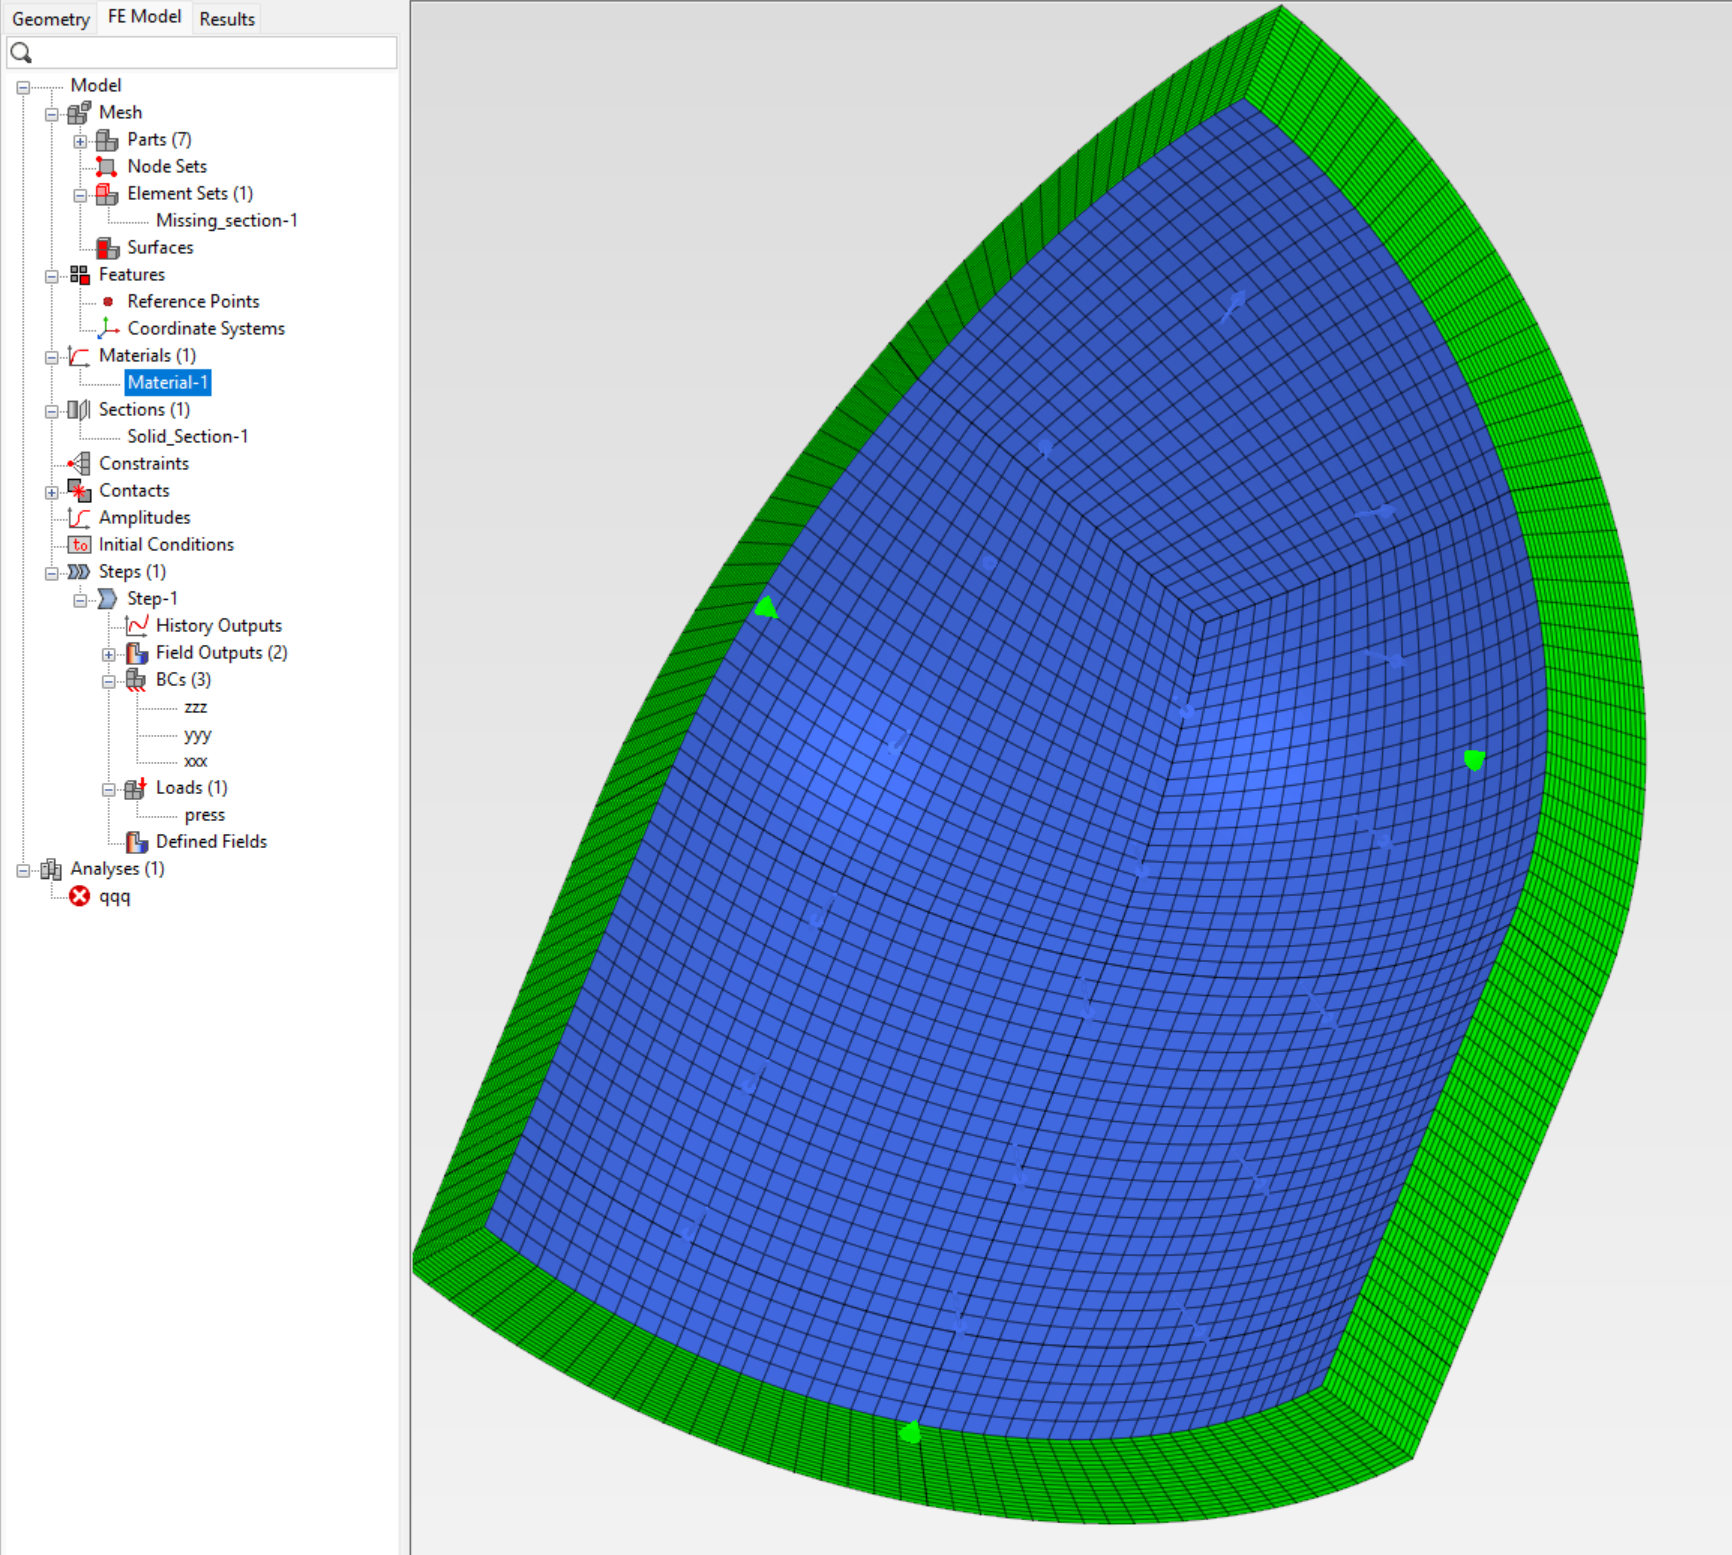
\includegraphics[keepaspectratio,scale=0.30]{images/sc14.png}}
            \only<2>{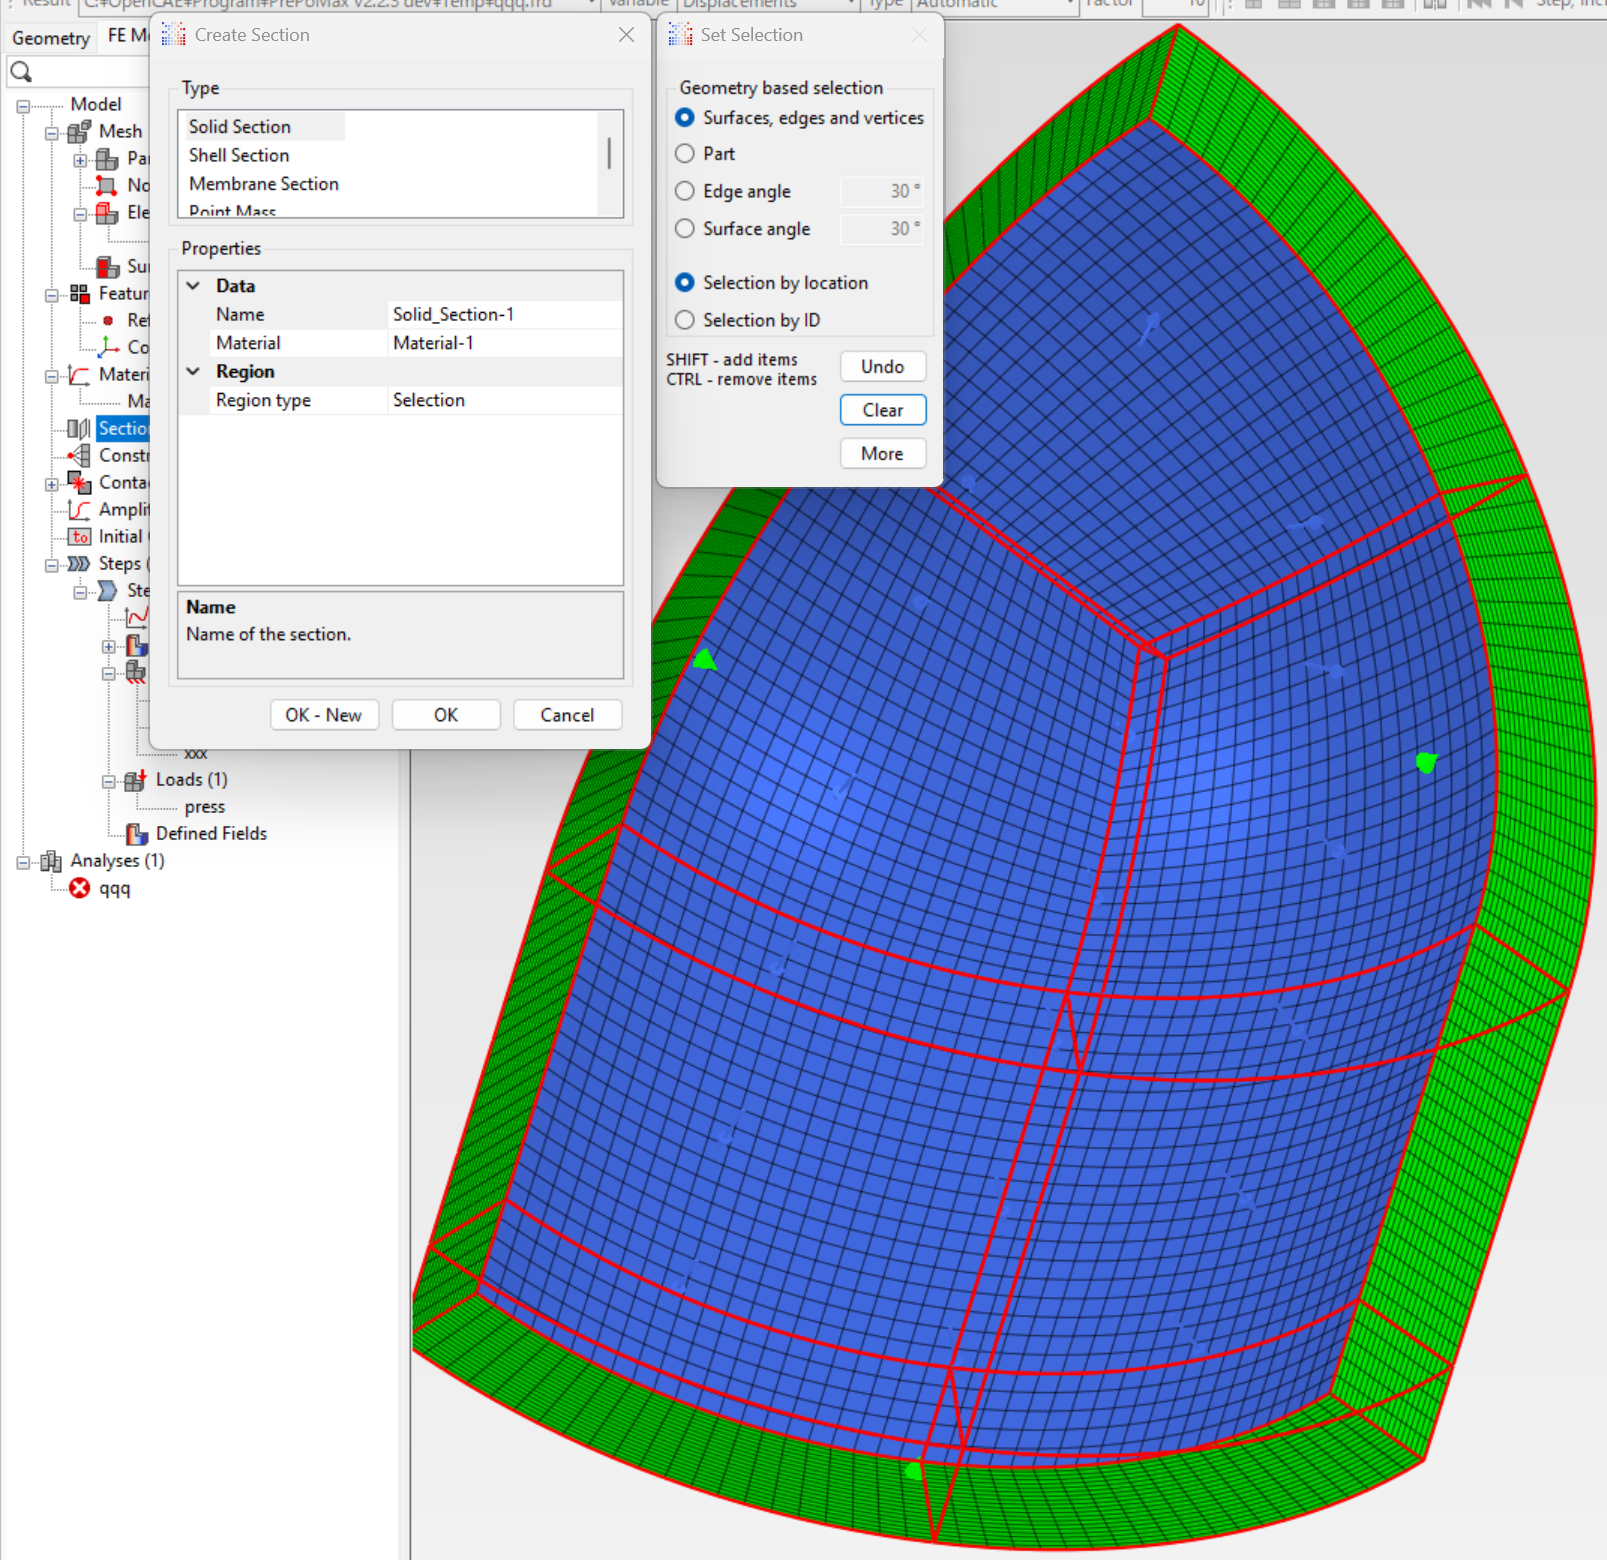
\includegraphics[keepaspectratio,scale=0.30]{images/sc15.png}}
            \caption{もろもろ作成の概要}
          \end{overlayarea}
        \end{center}
      \end{figure}
    \end{column}
  \end{columns}
  \only<1>{
    \begin{textblock*}{160pt}(200pt,70pt)
      \begin{tikzpicture}
         \node[rectangle,fill=cud_yellow,text width=90pt,text centered,rounded corners,minimum height=20pt](s) at (1cm,1cm) { \scriptsize 材質の作成};
         \draw[->, draw=cud_red, line width=1pt] (10pt,38pt) -- (42pt,110pt);
      \end{tikzpicture}
    \end{textblock*}
  }
  \only<2>{
    \begin{textblock*}{160pt}(195pt,42pt)
      \begin{tikzpicture}
         \node[rectangle,fill=cud_yellow,text width=90pt,text centered,rounded corners,minimum height=40pt](s) at (1cm,1cm) { \scriptsize Solid Section\\は 断面性状?};
         \draw[->, draw=cud_red, line width=1pt] (10pt,47pt) -- (55pt,114pt);
      \end{tikzpicture}
    \end{textblock*}
  }
\end{frame}
